\chapter{Choosing Industries for Wealth Creation}

This interview opens with a direct commercial question: if someone wants to create wealth in today's world, which industries deserve attention first? The answer is not a universal theory of entrepreneurship. It is a ranked field map: real estate, technology, and an industry one already understands. We should read the list as a practical sequence. First comes access, then judgment, then familiarity as a guardrail.

\paragraph{Source note.}
This chapter follows a School of Hard Knocks entrepreneurship interview curated for the LazyEarn track by LazyingArt LLC through Video2Book. The primary evidence is the spoken transcript.

\section{The Opening Wealth Question}

The interviewer begins by asking for the best three industries people should look at in order to create wealth. That question matters because it does not ask for a business idea, a tactic, or a motivational slogan. It asks for the arena.

An arena is where the entrepreneur will spend attention, capital, time, and error. Choosing it badly can make every later decision harder. Choosing it well does not guarantee success, but it gives the work a more favorable surface.

\subsection{Question \& Answer}

\paragraph{Question.}
What are the best three industries for someone trying to create wealth today?

\paragraph{Answer.}
The speaker gives a ranked answer:

\begin{enumerate}
\item Real estate.
\item Technology.
\item An industry that you already know something about.
\end{enumerate}

The ordering is the first useful point. We do not begin with the most glamorous category. We begin with a market the speaker sees as accessible, then move to a high-upside category that requires sharper judgment, and finally return to the learner's own knowledge base.

\begin{figure}
\centering
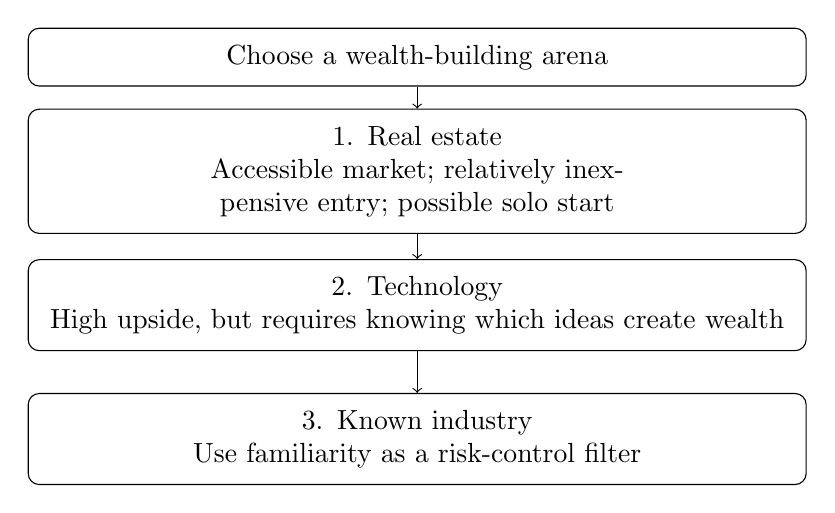
\begin{tikzpicture}[
  every node/.style={
    draw,
    rounded corners,
    align=center,
    text width=0.78\linewidth,
    inner sep=6pt
  }
]
\node (q) at (0,0) {Choose a wealth-building arena};
\node (r) at (0,-1.45) {1. Real estate\\Accessible market; relatively inexpensive entry; possible solo start};
\node (t) at (0,-3.15) {2. Technology\\High upside, but requires knowing which ideas create wealth};
\node (k) at (0,-4.85) {3. Known industry\\Use familiarity as a risk-control filter};
\draw[->] (q) -- (r);
\draw[->] (r) -- (t);
\draw[->] (t) -- (k);
\end{tikzpicture}
\caption{Transcript-derived decision sequence. This is a reconstruction of the spoken ranking, not a board diagram.}
\end{figure}

\section{Real Estate: Access First}

The first answer is real estate. The speaker calls it a fantastic market and emphasizes that one can get into it relatively inexpensively and do it by oneself.

The claim has two parts. The first is about the market: real estate is presented as a field worth entering. The second is about access: the speaker highlights the possibility of starting without a large organization around the entrepreneur. That is why real estate appears first. It answers the beginner's constraint before it answers the investor's ambition.

\begin{definition}[Accessible entry]
An industry has accessible entry, in the sense used here, when a beginner can plausibly begin learning and operating without needing a large team, a specialized technical staff, or institutional control from the outset.
\end{definition}

This definition is not a formal theorem. It is the practical mechanism behind the first recommendation. The speaker is saying, in effect, that a wealth-building arena should not merely be large. It should be enterable.

\section{Technology: Upside Requires Discernment}

The second answer is technology, but the speaker immediately qualifies it. Technology is not recommended as a blanket category. The warning is that one needs to know a lot about technology as it relates to which technologies will propel wealth and which may consume it.

That pivot is the center of the interview. Real estate is introduced through access. Technology is introduced through judgment. The danger is not that technology lacks opportunity; the danger is that opportunity and waste can look similar to the untrained eye.

\begin{remark}
The speaker's distinction between technologies that propel wealth and technologies that ``suck'' wealth should be preserved. It is vivid, but it is also analytical: some opportunities compound capital and attention, while others drain both.
\end{remark}

A clean note form is to treat technology as a filter problem:

\begin{itemize}
\item Some technology ideas are genuinely strong.
\item More technology ideas are weak, confused, or commercially dangerous.
\item The entrepreneur's task is to tell the difference before committing too much capital or time.
\end{itemize}

\section{The Filtering Problem}

The speaker says there are many great technology ideas, and even more terrible ones. The point is not anti-technology. It is anti-undisciplined selection.

We can summarize the working filter in a compact table. The table is not an equation and should not be treated as a scoring model. It is a note-taking device that preserves the transcript's order and contrast.

\begin{table}
\centering
\begin{tabular}{p{0.23\linewidth} p{0.34\linewidth} p{0.32\linewidth}}
\hline
Industry & Interview claim & Practical filter \\
\hline
Real estate & A strong market with relatively inexpensive entry & Can we begin operating and learning without excessive complexity? \\
Technology & Can build wealth, but only with judgment & Do we know enough to separate strong ideas from dangerous ones? \\
Known industry & Recommended because familiarity matters & Do we already understand the customers, work, risks, or economics? \\
\hline
\end{tabular}
\caption{A compact decision table reconstructed from the interview.}
\end{table}

\paragraph{A worked selection check.}
Suppose we are comparing three possible starting points: a small real-estate service, a technology idea we do not understand, and a business in a field where we already have experience. The transcript's logic does not tell us to chase the most exciting option. It tells us to ask three questions in order.

\begin{enumerate}
\item Can we enter the field without excessive cost or institutional dependence?
\item If the field is technology, do we understand why this idea should create wealth rather than consume it?
\item Do we know enough about the industry to recognize normal problems, bad assumptions, and real demand?
\end{enumerate}

Under that test, the unknown technology idea is not rejected automatically, but it cannot pass on excitement alone. It needs evidence and judgment. The familiar industry may deserve more attention than a fashionable category because the entrepreneur brings a working map of the terrain.

\section{An Industry You Know}

The third recommendation is an industry that you know something about. The speaker says this may be a little knowledge or a lot, but the instruction is to get into something already familiar.

This is the resolution of the earlier technology warning. If bad opportunities are often hard to distinguish from good ones, then familiarity becomes a practical defense. It helps the entrepreneur notice what outsiders miss: customer habits, hidden costs, operational friction, and the difference between a real need and an attractive story.

\begin{definition}[Familiarity filter]
The familiarity filter is the discipline of preferring arenas where the entrepreneur already has some direct knowledge, even if that knowledge is incomplete. It does not replace research, but it improves the first round of judgment.
\end{definition}

The speaker does not say that knowledge must be complete. That is important. A little familiarity can still be useful if it gives the beginner enough context to ask better questions and avoid the most obvious traps.

\section{Summary: Three Entries, One Filter}

The interview gives a short ranked answer, but the underlying structure is richer than a list. Real estate appears first because it is framed as accessible. Technology appears second because it can create wealth but demands discernment. A known industry appears third because familiarity controls risk.

The durable lesson is that wealth creation begins with arena selection. We choose where to play before we choose the exact move. The speaker's sequence gives us a practical order: start with access, respect judgment, and use familiarity as a filter against blind opportunity chasing.